\documentclass[preprint,12pt,aps,pra,showkeys,amsmath,amssymb,superscriptaddress,floatfix]{revtex4-2}
\usepackage[T1]{fontenc}
\usepackage[utf8]{inputenc}
\usepackage{amsmath,amssymb,amsthm,mathtools,mathrsfs}
\usepackage{microtype,booktabs,enumitem}
\usepackage{xcolor,tikz,etoolbox}
\usepackage[skins,breakable]{tcolorbox}
\usepackage{needspace}
% Keep diagram geometry independent of REVTeX preprint body spacing.
\AtBeginEnvironment{tikzpicture}{\linespread{1}\selectfont}
\usetikzlibrary{arrows.meta,positioning,calc,fit,decorations.pathreplacing}
\usepackage{graphicx}
\usepackage{hyperref}

\definecolor{MMBlue}{RGB}{0,82,155}
\definecolor{MMOrange}{RGB}{200,80,0}
\tikzset{
 mmnode/.style={draw=MMBlue,rounded corners=2pt,fill=MMBlue!4,align=left,execute at begin node={\raggedright},text width=5cm,font=\fontsize{10}{12}\selectfont,inner sep=6pt},
 mmimport/.style={mmnode,draw=black!65,fill=black!4},
 mmcandidate/.style={mmnode,draw=MMOrange,dashed,fill=MMOrange!5},
 mmrejected/.style={mmnode,draw=black,densely dotted,fill=black!8},
 mmproof/.style={->,thick,MMBlue},
 mmflow/.style={->,semithick,black!70},
 mmrepair/.style={->,dashed,thick,MMOrange},
 mmcandidatearrow/.style={->,dashed,semithick,MMOrange},
 mmnote/.style={font=\scriptsize,fill=white,inner sep=2pt,align=center}}

\usepackage[section]{placeins}
\setlength{\emergencystretch}{3em}
\setlist{itemsep=3pt,topsep=4pt}
\newtheorem{theorem}{Theorem}[section]
\newtheorem{proposition}[theorem]{Proposition}
\newtheorem{lemma}[theorem]{Lemma}
\newtheorem{corollary}[theorem]{Corollary}
\theoremstyle{definition}
\newtheorem{definition}[theorem]{Definition}
\newtheorem{example}[theorem]{Example}
\theoremstyle{remark}
\newtheorem{remark}[theorem]{Remark}
% Avoid isolated statement headings and single-line paragraph fragments.
\BeforeBeginEnvironment{theorem}{\Needspace{6\baselineskip}}
\BeforeBeginEnvironment{definition}{\Needspace{5\baselineskip}}
\BeforeBeginEnvironment{proposition}{\Needspace{5\baselineskip}}
\BeforeBeginEnvironment{lemma}{\Needspace{5\baselineskip}}
\BeforeBeginEnvironment{corollary}{\Needspace{5\baselineskip}}
\clubpenalty=5000
\widowpenalty=5000
\newcommand{\R}{\mathbb R}\newcommand{\Z}{\mathbb Z}\newcommand{\N}{\mathbb N}
\newcommand{\Pa}{\operatorname{Pa}}\newcommand{\Desc}{\operatorname{Desc}}
\newcommand{\cl}{\operatorname{cl}}\newcommand{\cost}{\operatorname{cost}}
\newcommand{\status}{\operatorname{status}}
% Faculty cards: a visual rail groups the five faculties within one agent.
% The rail has no arrowhead and does not represent a proof dependency.
\newcommand{\mmfacultybadge}[1]{%
 \node[circle,draw=MMBlue,line width=1pt,fill=white,
 minimum size=7mm,inner sep=0pt,font=\sffamily\small\bfseries,text=MMBlue]
 at ([xshift=15pt,yshift=-15pt]frame.north west) {#1};}
\newcommand{\mmfacultyrail}{%
 \draw[MMBlue!80,line width=1pt]
 ([xshift=15pt,yshift=2pt]frame.north west)--
 ([xshift=15pt,yshift=-2pt]frame.south west);}
\newtcolorbox{mmfacultybox}[2]{enhanced,breakable,
 colback=MMBlue!4,colframe=MMBlue!4,boxrule=0pt,arc=3pt,
 left=39pt,right=9pt,top=4pt,bottom=4pt,
 before skip=2pt,after skip=2pt,
 fontupper=\small\linespread{1.1}\selectfont,
 overlay unbroken={\mmfacultyrail\mmfacultybadge{#1}},
 overlay first={\mmfacultyrail\mmfacultybadge{#1}},
 overlay middle={\mmfacultyrail},overlay last={\mmfacultyrail}}
\newcommand{\mmfaculty}[3]{%
 \begin{mmfacultybox}{#1}{#2}
 {\sffamily\bfseries\color{MMBlue}#2}\par\smallskip #3
 \end{mmfacultybox}}
\newcommand{\agent}[9]{%
 \Needspace{8\baselineskip}
 \subsubsection{#1}
 \noindent\textbf{Object.} #2\par
 \noindent\textbf{Role.} #3\par\smallskip
 \mmfaculty{E}{Ego}{#4}
 \mmfaculty{M}{Memory}{#5}
 \mmfaculty{I}{Intellect}{#6}
 \mmfaculty{S}{Sense}{#7}
 \mmfaculty{A}{Action}{#8}
 \smallskip\noindent #9\par}

\usepackage{longtable,array,calc}
\providecommand{\tightlist}{\setlength{\itemsep}{2pt}\setlength{\parskip}{0pt}}
\makeatletter
\def\frontmatter@abstract@produce{\par\addvspace{\frontmatter@preabstractspace}%
\begingroup\prep@absbox\unvbox\absbox\post@absbox\endgroup
\addvspace{\frontmatter@postabstractspace}}
\makeatother
\newcommand{\field}[2]{\par\smallskip\noindent\textbf{#1.} #2\par}
\setlength{\emergencystretch}{5em}
\AtBeginEnvironment{verbatim}{\small\linespread{1.0}\selectfont}


\hypersetup{colorlinks=true,linkcolor=MMBlue,urlcolor=MMBlue,pdfauthor={Dibakar Sigdel}}

\begin{document}

\title{Residue Theorem\\[4pt]\large An End-to-End Meta-Math Walkthrough}

\author{Dibakar Sigdel}

\affiliation{Mindverse Computing LLC, Lynnwood, WA 98087, USA}

\date{October 2026}

\begin{abstract}

A complete authored walkthrough of residue theorem, with explicit
mathematical contracts, local verification gates, and reusable exports.
The report presents the target theorem, declared imports, a dependency
graph, five-faculty node contracts, a continuous proof, a worked
example, and a hypothesis-repair audit. It is an authored mathematical
exposition, not a deployed-agent transcript or a formal proof-assistant
certificate.

\end{abstract}\maketitle\linespread{1.12}\selectfont

\noindent\textbf{CA-03 / Complex Analysis / Report v1}

\section{Target and import contract}

\begin{theorem}

Let D be a bounded Jordan domain whose positively oriented boundary
gamma is piecewise smooth. Let f be holomorphic in an open neighborhood
of the closure of D except for finitely many isolated singularities
\(a_1,\ldots,a_s\) inside D. Then

\[\oint_\gamma f(z)\,dz=2\pi i\sum_{j=1}^s\operatorname{Res}(f,a_j).\]

The output is a contour identity with all interior singularities
included. Singularities on the contour are excluded. Essential isolated
singularities are allowed; the theorem does not require every
singularity to be a pole.

\end{theorem}

\subsection{Foundations and permitted imports}

a residue is the coefficient of \((z-a)^{-1}\) in the Laurent expansion;
positive outer orientation is counterclockwise. Import the Laurent
expansion theorem and uniform convergence on compact annuli. Import
Cauchy--Goursat's boundary form: a function holomorphic near a finitely
connected region's closure has zero integral around its full oriented
boundary. This follows by cuts or subdivision into simply connected
pieces with cancellation of internal sides; it is not the residue
theorem being proved.

\clearpage\section{Node interaction workflow}

\begin{center}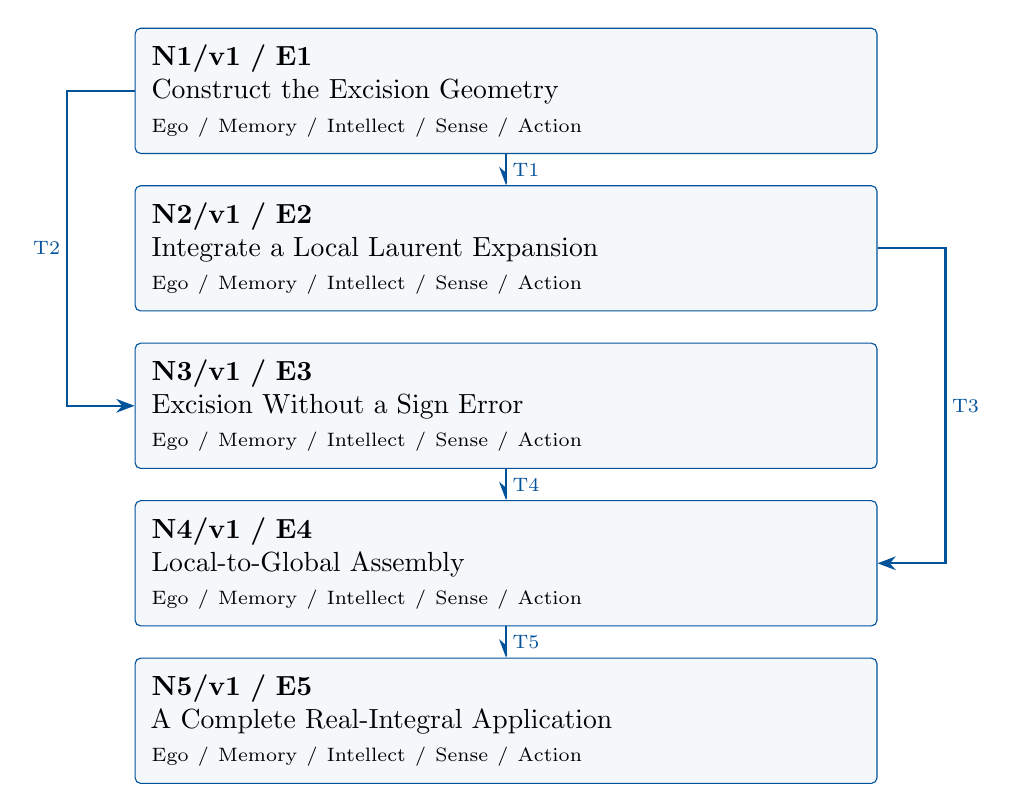
\begin{tikzpicture}[>=Stealth,x=1cm,y=1cm]

\node[mmnode,text width=9cm,minimum height=1.25cm] (N1) at (0,0.0) {\textbf{N1/v1 / E1}\\Construct the Excision Geometry\\{\scriptsize Ego / Memory / Intellect / Sense / Action}};

\node[mmnode,text width=9cm,minimum height=1.25cm] (N2) at (0,-2.0) {\textbf{N2/v1 / E2}\\Integrate a Local Laurent Expansion\\{\scriptsize Ego / Memory / Intellect / Sense / Action}};

\node[mmnode,text width=9cm,minimum height=1.25cm] (N3) at (0,-4.0) {\textbf{N3/v1 / E3}\\Excision Without a Sign Error\\{\scriptsize Ego / Memory / Intellect / Sense / Action}};

\node[mmnode,text width=9cm,minimum height=1.25cm] (N4) at (0,-6.0) {\textbf{N4/v1 / E4}\\Local-to-Global Assembly\\{\scriptsize Ego / Memory / Intellect / Sense / Action}};

\node[mmnode,text width=9cm,minimum height=1.25cm] (N5) at (0,-8.0) {\textbf{N5/v1 / E5}\\A Complete Real-Integral Application\\{\scriptsize Ego / Memory / Intellect / Sense / Action}};

\draw[mmproof] (N1.south) -- node[mmnote,right] {T1} (N2.north);

\draw[mmproof] (N1.west) -- (-5.58,0) -- node[mmnote,left] {T2} (-5.58,-4) -- (N3.west);

\draw[mmproof] (N2.east) -- (5.58,-2) -- node[mmnote,right] {T3} (5.58,-6) -- (N4.east);

\draw[mmproof] (N3.south) -- node[mmnote,right] {T4} (N4.north);

\draw[mmproof] (N4.south) -- node[mmnote,right] {T5} (N5.north);

\end{tikzpicture}\end{center}

Each box is one mathematical agent containing all five faculties. Blue
arrows carry the versioned exports listed below. The layout gives a
reading order; only drawn arrows assert dependencies. Diagnostic repair
is separate from the proof DAG.

\clearpage\subsection{Versioned evidence-transfer ledger}

\begingroup\small\linespread{1.05}\selectfont

\Needspace{5\baselineskip}\field{T1: N1/E1/v1 to N2}{Every isolated interior singularity has a disjoint closed isolating disk
lying in the domain.}

\field{Receiving activity}{N2: Integrate a Local Laurent Expansion}

\field{Compatibility}{Use the same mathematical objects and hypotheses as the source export.
Receiving contract: N1/E1 and the Laurent expansion on each punctured
disk, uniformly convergent on the circle.}

\Needspace{5\baselineskip}\field{T2: N1/E1/v1 to N3}{Every isolated interior singularity has a disjoint closed isolating disk
lying in the domain.}

\field{Receiving activity}{N3: Excision Without a Sign Error}

\field{Compatibility}{Use the same mathematical objects and hypotheses as the source export.
Receiving contract: N1/E1 and Cauchy--Goursat for the region with the
disks removed.}

\Needspace{5\baselineskip}\field{T3: N2/E2/v1 to N4}{\(\oint_{C_j}f(z)\,dz=2\pi i\,\operatorname{Res}(f,a_j)\) for each
counterclockwise local circle.}

\field{Receiving activity}{N4: Local-to-Global Assembly}

\field{Compatibility}{Use the same mathematical objects and hypotheses as the source export.
Receiving contract: N2/E2 for every singularity and N3/E3 for the same
contour.}

\Needspace{5\baselineskip}\field{T4: N3/E3/v1 to N4}{\(\oint_\gamma f=\sum_j\oint_{C_j}f\).}

\field{Receiving activity}{N4: Local-to-Global Assembly}

\field{Compatibility}{Use the same mathematical objects and hypotheses as the source export.
Receiving contract: N2/E2 for every singularity and N3/E3 for the same
contour.}

\Needspace{5\baselineskip}\field{T5: N4/E4/v1 to N5}{\(\oint_\gamma f(z)\,dz=2\pi i\sum_j\operatorname{Res}(f,a_j)\).}

\field{Receiving activity}{N5: A Complete Real-Integral Application}

\field{Compatibility}{Use the same mathematical objects and hypotheses as the source export.
Receiving contract: N4/E4 for upper semicircles of radius \(R>1\);
elementary improper integration.}

\endgroup

\clearpage\section{Agent roles and five-faculty activities}\begingroup\small\linespread{1.05}\selectfont\setlist{itemsep=1pt,topsep=2pt}

\subsection{N1/v1: Construct the Excision Geometry}

\field{Object and role}{Construct the Excision Geometry. Establish the following local result:
Every isolated interior singularity has a disjoint closed isolating disk
lying in the domain.}

\field{Inputs}{A positively oriented piecewise smooth Jordan boundary; finitely many
isolated interior singularities and none on the boundary.}

\mmfaculty{E}{Ego}{Own E1/v1: Every isolated interior singularity has a disjoint closed
isolating disk lying in the domain.}

\mmfaculty{M}{Memory}{Holomorphic domain and singularities}

\mmfaculty{I}{Intellect}{Choose disjoint local disks}

\mmfaculty{S}{Sense}{Exclude boundary singularities}

\mmfaculty{A}{Action}{Carry out the numbered deductions and publish E1/v1 together with its
hypotheses and proof location.}

\smallskip\noindent\textbf{Numbered mathematical activities}

\begin{enumerate}[label=N1.\arabic*,leftmargin=3.4em]

\item Use finiteness and interiority to choose disjoint small disks.

\item Keep their boundaries away from singularities.

\item Record the outer orientation and the counterclockwise local-circle
conventions.

\end{enumerate}

\field{Export E1/v1}{Every isolated interior singularity has a disjoint closed isolating disk
lying in the domain.}

\field{Acceptance gate}{Exclude boundary singularities Publish only after checking every
displayed deduction.}

\field{Targeted repair}{If the check fails, revise N1: Exclude boundary singularities Recheck
dependent nodes N2, N3, N4, N5.}

\clearpage

\subsection{N2/v1: Integrate a Local Laurent Expansion}

\field{Object and role}{Integrate a Local Laurent Expansion. Establish the following local
result: \(\oint_{C_j}f(z)\,dz=2\pi i\,\operatorname{Res}(f,a_j)\) for
each counterclockwise local circle.}

\field{Inputs}{N1/E1 and the Laurent expansion on each punctured disk, uniformly
convergent on the circle.}

\mmfaculty{E}{Ego}{Own E2/v1: \(\oint_{C_j}f(z)\,dz=2\pi i\,\operatorname{Res}(f,a_j)\) for
each counterclockwise local circle.}

\mmfaculty{M}{Memory}{N1/E1 and the Laurent expansion on each punctured disk, uniformly
convergent on the circle.}

\mmfaculty{I}{Intellect}{Integrate a Local Laurent Expansion.}

\mmfaculty{S}{Sense}{Check the hypotheses and each step of the displayed calculation.}

\mmfaculty{A}{Action}{Carry out the numbered deductions and publish E2/v1 together with its
hypotheses and proof location.}

\smallskip\noindent\textbf{Numbered mathematical activities}

\begin{enumerate}[label=N2.\arabic*,leftmargin=3.4em]

\item Integrate the Laurent series term by term on the compact circle.

\item Parametrize \(z=a_j+r e^{it}\) and integrate each integer power.

\item Only the coefficient of \((z-a_j)^{-1}\) contributes; poles and
essential isolated singularities are both covered.

\end{enumerate}

\field{Export E2/v1}{\(\oint_{C_j}f(z)\,dz=2\pi i\,\operatorname{Res}(f,a_j)\) for each
counterclockwise local circle.}

\field{Acceptance gate}{Check the hypotheses and each step of the displayed calculation. Publish
only after checking every displayed deduction.}

\field{Targeted repair}{If the check fails, revise N2: Check the hypotheses and each step of the
displayed calculation. Recheck dependent nodes N4, N5.}

\clearpage

\subsection{N3/v1: Excision Without a Sign Error}

\field{Object and role}{Excision Without a Sign Error. Establish the following local result:
\(\oint_\gamma f=\sum_j\oint_{C_j}f\).}

\field{Inputs}{N1/E1 and Cauchy--Goursat for the region with the disks removed.}

\mmfaculty{E}{Ego}{Own E3/v1: \(\oint_\gamma f=\sum_j\oint_{C_j}f\).}

\mmfaculty{M}{Memory}{Cauchy--Goursat boundary form}

\mmfaculty{I}{Intellect}{Remove singularity disks}

\mmfaculty{S}{Sense}{Track clockwise hole boundaries}

\mmfaculty{A}{Action}{Carry out the numbered deductions and publish E3/v1 together with its
hypotheses and proof location.}

\smallskip\noindent\textbf{Numbered mathematical activities}

\begin{enumerate}[label=N3.\arabic*,leftmargin=3.4em]

\item Apply the boundary theorem where \(f\) is holomorphic.

\item Inner boundaries are clockwise in the punctured domain.

\item Move their negatives to the other side, leaving counterclockwise local
integrals.

\end{enumerate}

\field{Export E3/v1}{\(\oint_\gamma f=\sum_j\oint_{C_j}f\).}

\field{Acceptance gate}{Track clockwise hole boundaries Publish only after checking every
displayed deduction.}

\field{Targeted repair}{If the check fails, revise N3: Track clockwise hole boundaries Recheck
dependent nodes N4, N5.}

\clearpage

\subsection{N4/v1: Local-to-Global Assembly}

\field{Object and role}{Local-to-Global Assembly. Establish the following local result:
\(\oint_\gamma f(z)\,dz=2\pi i\sum_j\operatorname{Res}(f,a_j)\).}

\field{Inputs}{N2/E2 for every singularity and N3/E3 for the same contour.}

\mmfaculty{E}{Ego}{Own E4/v1:
\(\oint_\gamma f(z)\,dz=2\pi i\sum_j\operatorname{Res}(f,a_j)\).}

\mmfaculty{M}{Memory}{All local certificates}

\mmfaculty{I}{Intellect}{Sum independent local contributions}

\mmfaculty{S}{Sense}{Include every singularity}

\mmfaculty{A}{Action}{Carry out the numbered deductions and publish E4/v1 together with its
hypotheses and proof location.}

\smallskip\noindent\textbf{Numbered mathematical activities}

\begin{enumerate}[label=N4.\arabic*,leftmargin=3.4em]

\item Substitute every local residue integral into the excision identity.

\item Check no singularity is omitted or counted twice.

\item With no singularities the empty sum recovers Cauchy--Goursat.

\end{enumerate}

\field{Export E4/v1}{\(\oint_\gamma f(z)\,dz=2\pi i\sum_j\operatorname{Res}(f,a_j)\).}

\field{Acceptance gate}{Include every singularity Publish only after checking every displayed
deduction.}

\field{Targeted repair}{If the check fails, revise N4: Include every singularity Recheck
dependent nodes N5.}

\clearpage

\subsection{N5/v1: A Complete Real-Integral Application}

\field{Object and role}{A Complete Real-Integral Application. Establish the following local
result: \(\int_{-\infty}^{\infty}(1+x^2)^{-1}\,dx=\pi\).}

\field{Inputs}{N4/E4 for upper semicircles of radius \(R>1\); elementary improper
integration.}

\mmfaculty{E}{Ego}{Own E5/v1: \(\int_{-\infty}^{\infty}(1+x^2)^{-1}\,dx=\pi\).}

\mmfaculty{M}{Memory}{Contour identity and decay estimates}

\mmfaculty{I}{Intellect}{Separate real and arc integrals}

\mmfaculty{S}{Sense}{Audit improper limit}

\mmfaculty{A}{Action}{Carry out the numbered deductions and publish E5/v1 together with its
hypotheses and proof location.}

\smallskip\noindent\textbf{Numbered mathematical activities}

\begin{enumerate}[label=N5.\arabic*,leftmargin=3.4em]

\item The sole enclosed pole is \(i\), with residue \(1/(2i)\).

\item Bound the arc integral by \(\pi R/(R^2-1)\), which tends to zero.

\item Use absolute integrability on the real axis and take the radius limit.

\end{enumerate}

\field{Export E5/v1}{\(\int_{-\infty}^{\infty}(1+x^2)^{-1}\,dx=\pi\).}

\field{Acceptance gate}{Audit improper limit Publish only after checking every displayed
deduction.}

\field{Targeted repair}{If the check fails, revise N5: Audit improper limit Withhold this
terminal result until its gate passes.}

\endgroup\clearpage\section{Continuous mathematical proof}\label{sec:proof}

\subsection{N1 --- Construct the Excision
Geometry}\label{n1-construct-the-excision-geometry}

Choose small closed disks around the \(a_j\), disjoint from one another
and contained in D, with no other singularity in any disk. Let \(C_j\)
be the positively oriented circle bounding the jth disk. Their radii can
be chosen because the singularity list is finite and each point is
isolated.

\subsection{N2 --- Integrate a Local Laurent
Expansion}\label{n2-integrate-a-local-laurent-expansion}

Write \(f(z)=\sum_{k\in\mathbb Z}c_k(z-a_j)^k\) in the punctured local
neighborhood. Uniform convergence on \(C_j\) justifies termwise
integration. Parameterizing \(z=a_j+re^{it}\) yields

\[\oint_{C_j}(z-a_j)^k\,dz=\begin{cases}2\pi i&k=-1,\\0&k\ne-1.\end{cases}\]

For \(k\ne -1\) the exponential \(e^{i(k+1)t}\) integrates to zero; for
\(k=-1\) the integrand times dz is i dt. Therefore
\(\oint_{C_j}f=2\pi i c_{-1}=2\pi i\operatorname{Res}(f,a_j)\).

\subsection{N3 --- Excision Without a Sign
Error}\label{n3-excision-without-a-sign-error}

Remove the disk interiors from D. The resulting region has boundary
gamma together with the hole circles in clockwise orientation.
Cauchy--Goursat applies because every singularity has been excised.
Hence

\[0=\oint_\gamma f-\sum_j\oint_{C_j}f.\]

Thus the outer contour integral equals the sum of the counterclockwise
local integrals. An inner circle's orientation is reversed in the region
boundary; the minus sign is part of the proof.

\subsection{N4 --- Local-to-Global
Assembly}\label{n4-local-to-global-assembly}

Substitute the N2 certificates into the N3 identity. This gives exactly
the theorem. With no singularities, the sum is empty and the result
reduces to Cauchy--Goursat. \(\square\)

\subsection{N5 --- A Complete Real-Integral
Application}\label{n5-a-complete-real-integral-application}

For \(f(z)=1/(1+z^2)\), take the real segment from \(-R\) to R followed
by the upper semicircle, \(R>1\). The only interior pole is i, with

\[\operatorname{Res}(f,i)=\lim_{z\to i}\frac{z-i}{(z-i)(z+i)}=\frac1{2i}.\]

The contour integral is therefore pi. On the arc, \(|1+z^2|\ge R^2-1\)
and its length is pi R, giving

\[\left|\int_{\mathrm{arc}}\frac{dz}{1+z^2}\right|\le\frac{\pi R}{R^2-1}\longrightarrow0.\]

The real integrand is absolutely integrable: it is bounded near zero and
at most \(1/x^2\) for \(|x|\ge 1\). Passing to the improper limit gives

\[\int_{-\infty}^{\infty}\frac{dx}{1+x^2}=\pi.\]

A residue calculation alone would not justify this conclusion without
the arc estimate and existence of the real improper integral.

\hfill$\square$

\section{Worked orchestration}

Take \(f(z)=(z+1)/((z-1)(z-2))\) on \(|z|=3\), positively oriented. The
two local agents independently obtain

\[\operatorname{Res}(f,1)=\frac2{-1}=-2,\qquad\operatorname{Res}(f,2)=\frac3{1}=3.\]

N4 sums them to 1, so the contour integral is \(2\pi i\). Both poles
must be included even though their contributions partially cancel.

\begin{itemize}
\item
  \textbf{Interaction}

  N1 \(\to\) local agents

  \textbf{Evidence transferred}

  Disjoint analytic neighborhoods at 1 and 2
\item
  \textbf{Interaction}

  Local agent 1 \(\to\) N4

  \textbf{Evidence transferred}

  Residue \(-2\) with simple-pole calculation
\item
  \textbf{Interaction}

  Local agent 2 \(\to\) N4

  \textbf{Evidence transferred}

  Residue 3 with simple-pole calculation
\item
  \textbf{Interaction}

  N3 \(\to\) N4

  \textbf{Evidence transferred}

  Outer integral equals sum of positively oriented local integrals
\item
  \textbf{Interaction}

  N4 \(\to\) caller

  \textbf{Evidence transferred}

  Total residue 1 and contour integral \(2\pi i\)
\end{itemize}

\subsection{Boundary and hypothesis audit}

\begin{itemize}
\tightlist
\item
  Reversing the outer orientation reverses the integral's sign.
\item
  Higher-order poles still use the Laurent coefficient, not the
  simple-pole limit formula.
\item
  A removable singularity has residue zero.
\item
  Arc decay must be proved for the chosen function and contour.
\item
  A plot or sampled singularity search does not establish the exhaustive
  pole list.
\end{itemize}

Export the local Laurent-integral lemma, the excision identity, the
finite-singularity residue theorem, and the rational-integral
application. These modules support the argument principle and Rouché's
theorem in the problem bank.

\section{Illustrative failure and repair}

The following is an authored diagnostic scenario. Changed assumptions
define a new contract; they do not retroactively prove the original
statement.

\subsection{Failure and correction}
Suppose a branch uses \(|z|=1\) for \(1/(1+z^{2})\). Both poles lie on
the contour; the theorem's contract fails.

\begin{itemize}
\item
  \textbf{Node:} N1
\item
  \textbf{State:} STALLED
\item
  \textbf{Failing faculty:} Sense
\item
  \textbf{Failed hypothesis:} no singularities on contour
\item
  \textbf{Observed:} poles i and -i on \(|z|=1\)
\item
  \textbf{Repair target:} contour selection
\item
  \textbf{Blocked export:} ordinary residue-theorem contour integral
\end{itemize}

Memory retrieves the domain hypothesis. Sense identifies both boundary
poles. Intellect selects \(|z|=2\) for a revised problem. Action checks
both poles are interior and computes residues 1/(2i) and \(-1/(2i)\),
whose sum is zero. Ego exports integral zero for the revised contour. An
indented contour or principal value would be a different problem
requiring additional analysis.

\subsection{Hypothesis boundary}
\begin{itemize}
\tightlist
\item
  Reversing the outer orientation reverses the integral's sign.
\item
  Higher-order poles still use the Laurent coefficient, not the
  simple-pole limit formula.
\item
  A removable singularity has residue zero.
\item
  Arc decay must be proved for the chosen function and contour.
\item
  A plot or sampled singularity search does not establish the exhaustive
  pole list.
\end{itemize}

Export the local Laurent-integral lemma, the excision identity, the
finite-singularity residue theorem, and the rational-integral
application. These modules support the argument principle and Rouché's
theorem in the problem bank.

\subsection{Version and recheck}
Treat any changed assumption as a new contract. Recheck the revised
export and all of its descendants. A backward diagnostic never
establishes an earlier theorem. This is an authored teaching trace, not
an execution log.

\par\medskip\begingroup\small\linespread{1.0}\selectfont\noindent\textbf{Provenance.} This authored proof is complete relative to its declared imports. Reuse
each export with its assumptions, proof, and version. The original
Markdown remains available for comparison.
\par\endgroup

\par\smallskip\begingroup\small\linespread{1.0}\selectfont\noindent\textbf{Further reading.} \href{https://people.math.harvard.edu/~siu/math113/}{Harvard complex
analysis, Laurent series and residue theorem lectures}.\par\endgroup

\end{document}
